\documentclass{beamer}
\usepackage{graphicx}
\usepackage{amsfonts, amsmath, amssymb}
\usepackage{algorithm}
\usepackage{algpseudocode}
\usepackage{float}
\usepackage{animate}
\usepackage{tikz}
\usepackage{multimedia}
\setbeamercovered{transparent}
\title{Q Learning and Deep Q Network}
\author{Ling Fei Zhang\\
    260985358}

\usetheme{Darmstadt}
\usecolortheme{seahorse}

\begin{document}
\maketitle

\begin{frame}
    \frametitle{Table of Contents}
    \tableofcontents
\end{frame}

\section{Introduction}

\begin{frame}
    \frametitle{Games}
    \begin{columns}
        \column{0.5\textwidth}
        \centering
        CartPole
        \medskip
        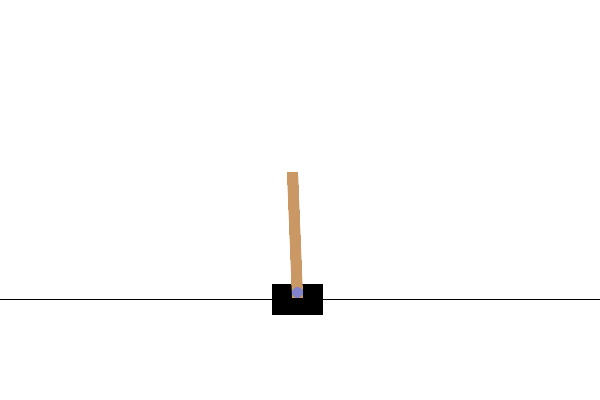
\includegraphics[width=\textwidth]{cart_pole.png}
        \column{0.5\textwidth}
        \centering
        Lunar Lander
        \medskip
        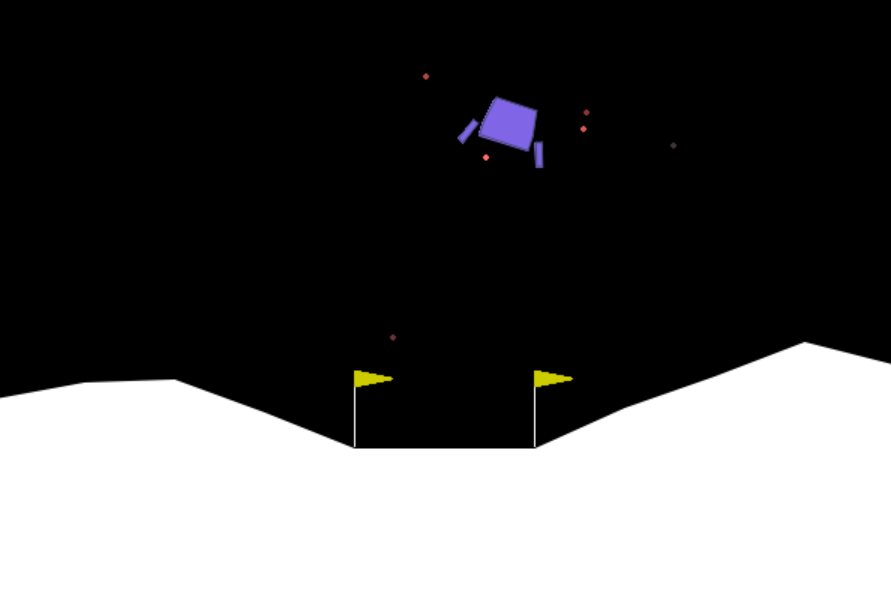
\includegraphics[width=\textwidth]{lunar.png}
    \end{columns}
\end{frame}

\begin{frame}
    \frametitle{Agents}
    \begin{itemize}
        \item Q Learning \pause
              \begin{itemize}
                  \item Model-free reinforcement learning algorithm \pause
                  \item Uses a table to store Q values for each state-action pair \pause
                  \item Effective in simple environments\pause
                  \item Struggles in more complexe environments since it is impractical to store and
                        update Q values for all the state-action pairs\pause
              \end{itemize}
        \item Deep Q Network (DQN) \pause
              \begin{itemize}
                  \item Uses neural networks to learn policies to map states to Q values\pause
                  \item Neural networks can handle large state spaces and continuous action spaces
              \end{itemize}
    \end{itemize}
\end{frame}

\section{Background}
\begin{frame}
    \frametitle{Background}

\end{frame}

\end{document}